\chapter{Introduction}
\label{chp:introduction}

\section{Context}
The remarkably complex and dynamic nature of the photosphere (the layer of the sun's atmosphere visible to the eye) allows for the accumulation of magnetic field in clustered areas known as "Active Regions" (ARs). Over time, as these regions grow, the magnetic field lines intertwine, forming magnetic flux ropes. These flux ropes are a collection of magnetic field lines and active plasma from the sun's surface that, if large enough, erupt to produce solar flares. When these eruptions are energetic, they release a large mass of plasma and magnetic field into interplanetary space known as a Coronal Mass Ejection (CME). Naturally, being able to predict when a solar eruption occurs is of utmost importance for the prediction of "Space Weather" near earth. When CMEs impact the earth's magnetosphere, the ensuing geomagnetic storms cause a large current and magnetic field to propagate through the ionosphere, causing the upper atmosphere to expand, increasing drag on satellites, and causing currents to surge through long conductors on the ground like the power grid. The power grid picks these geomagnetically induced currents up, which can cause blackouts and damage to our electrical infrastructure. 

Some flare prediction in the past has involved classification based on physical properties such as $H_{\alpha}$ bands \cite{hale_magnetic_1919}, or the Ising number of the most active magnetic regions \cite{MCintosh}. Mathematical models such as the one described by Heyvaerts et al. \cite{heyvaerts_mathematical_1983} analyze the asymptotic behavior of solar flares as a series of partial differential equations, or the static solutions of magnetohydrodynamical systems of partial differential equations. Other visually-based forecasting methods exist, such as the McIntosh scale \cite{MCintosh}, which takes the visual characteristics of an AR and matches them to a look-up table of climatalogical flaring probability. \\

However, the above physical and visual feature-based forecasting methods fall short in that they are either highly simplified physical models or too sensitive to initial conditions and the seemingly chaotic surface of the sun makes it hard to propagate results through time. Physical models such as the CSHKP model \cite{choudhary_strassmeier_2011} of magnetic reconnection treat a flare as an idealized magnetic field that remains static in time. Mathematical models often assume a force-free magnetic field and quasi-static evolution, a harsh oversimplification.

A recent innovation in Flare prediction is Topological Data Analysis which analyzes the mathematical shape of an AR. The number of holes and components in an AR can be used as a feature in machine learning models. Because of the flexibility of modern neural networks, it is possible to design an algorithm, find more features (topological, geometric, and physical in this case), then inject them as inputs to prediction-based machine learning models without actually changing much of the underlying algorithm. Topological Data Analysis of ARs could yield insight into when ARs grow in complexity and how they evolve. The success of topological data analysis hints that their unique sub-regions better describe ARs. A ``hole" in an AR is simply a more dense \textbf{connected} subset of the magnetic field. Therefore, rather than heuristically measuring topological properties, I have chosen to define what a connected subset actually is in an AR (which I have defined to be an umbra/penumbra combination). Extracting this region and running similar tests as have been done before to the entire AR will result in better performance than simply extracting physical features from the entire AR. 

\section{Relevant Work}
\label{relevantworkchap}

Recently, flare forecasting methods have seen an uptick, with many reviews on the effectiveness and accuracy of each method (see \cite{Comparison1} \cite{Comparison2} \cite{Comparison3} \cite{Comparison4}). Deshmukh et al. \cite{varad} use Topological Data Analysis (TDA) to forecast flares and makes use of persistent homology diagrams to measure the number and prominence of topological ``1-holes" in an AR magnetogram. This method motivates my thesis because the segmentation of an AR into distinct subregions takes topological information (holes and subregions) and computes physical features for each isolated region. Deshmukh et al. extracts topological features (in the form of a persistence diagram) and passes this vector through a four-layer Artificial Neural Network (ANN) constructed using PyTorch \cite{pytorch}. Compared to the same neural network with 19 different SHARP features (on the entire AR), the topological approach performed just as well as the physics-based featurization. The topological feature set alone resulted in a $0.90 \pm 0.01$ accuracy, and the SHARP parameterization resulted in a $0.89 \pm 0.01$ accuracy. Note that \textit{accuracy} is defined as the number of correct predictions (true positives plus true negatives) over the total number of attempted predictions. There are better scoring methods (see chapter \ref{chaptermethods}) that take into account a large number of non-flaring regions within the feature set. \footnote{In fact, the Heidke skill score (the score I will use to address this problem) of Deshmukh et al. model using topology alone is $0.16 \pm 0.02$ where the SHARP features are lower at $0.13 \pm 0.01$}.

% TODO
This problem is inherently three-dimensional (as opposed to the data provided by the Solar Dynamics Observatory (SDO), which are images of the photospheric surface rather than the three-dimensional samples. Many methods attempt to describe the three-dimensional nature of AR to predict magnetic reconnection. Georgoulis et al. \cite{georgoulis_rust_2007} uses a method that measures the effective magnetic field ($B_{eff}$) in order to predict coronal connectivity as a metric for flaring.

On the other hand, removing the three-dimensional restriction based on a ``force-free" or zero net current models, it is hypothesized by Lekka et al. \cite{Properties1} that the parameterization of the solar surface using various physical metrics (total unsigned flux, total magnetic twist, etc.) is an efficient method for flare forecasting. Choudhary et al. \cite{choudhary_strassmeier_2011} and Yuan et al. \cite{yuan_shih_jing_wang_2010} use a method that computes total magnetic unsigned flux (one of the highest indications of flaring), length of the neutral line and total magnetic energy dissipation and uses this data with various machine learning methods. Similarly, Falconer et al. \cite{falconer_moore_gary_2008} measure the free magnetic energy inside strong gradient neutral lines and then use least squares to convert this distribution through Poisson statistics. This method works best for flares of class C1 or more. Using the same strong gradient neutral lines as a restricted domain, Schrijver \cite{schrijver} measures the magnetic field close to non-potential high gradient neutral lines in order to compute the $R$ parameter - the total adjacent flux to polarity inversion lines. In another primary motivation for this paper, Barnes et al. \cite{Properties1} measures many AR physical scalar quantities and performs a discriminant analysis to cluster flaring and non-flaring regions. The third paper of Barnes et al. \cite{Properties3} describes Magnetic Charge Topology (MCT) and partitions flux based on the primary charge sign. They use the current free potential to simulate coronal connections and magnetic reconnection.

Other non-physical features that measure more of the geometry of the AR have been used, such as the capacity or fractal dimension of the umbra and penumbra in Mcateer et al. \cite{mcateer_gallagher_conlon_2010}. This feature is motivated by flares that often occur in twisted and complicated-looking boundaries between highly positive and negative regions. The capacity dimension prescribes a metric to this property. Higgins et al. \cite{higgins_gallagher_mcateer_bloomfield_2011} produced another geometric approach to parameterization, designing Solar Monitor Active Region Tracker (SMART) to measure the area and flux of ARs as well as spatial properties and length of the neutral line, SMART feeds these parameters through a machine learning algorithm as features. Visual geometric properties have been encoded in the classical McIntosh \cite{MCintosh} classification system. The McIntosh class of an AR, as well as how this class changes through time, has been used in Automated Solar Activity Prediction (ASAP) \cite{colak_qahwaji_2007} \cite{colak_qahwaji_2009}. Colak et al. use the McIntosh class as a parameter for logistic regression and support vector machines.

The methods above have been used alone and in ensemble to predict flares. However, the Space Weather Prediction Center (SWPC) uses a team of educated forecasters who examine ARs by eye and categorize them based on their McIntosh \cite{MCintosh} scale.  \cite{VerificationCurrentMethod} conducts a review of the efficiency of this method, but it is very subjective. It was shown in \cite{VerificationCurrentMethod} that forecaster experience affects their decision accuracy, which is typically only slightly above simply labeling all images as non-flaring, even for experienced forecasters.

\section{Problem Space}
\label{sec:problemspace}

NASA's Solar Dynamics Observatory satellite has collected magnetograms (a measure of the magnetic field strength of the photosphere) and continuum intensity images of the entire solar disk (the area of the sun that faces earth) approximately every 12 minutes since 2010. Stanford's Joint Science Operations Center (JSOC) has created a pipeline that scans for ARs, regions with a greater total magnetic field. JSOC defines cut-out regions around ARs as Space weather HMI Region Patches (SHARPs) \cite{SHARP_Pipeline}. JSOC organizes SHARPs by distinct HMI Region Patch Number (HARP Number) (a unique number that labels that AR as it moves across the solar disk) and a timestamp that encodes the time of the image. So a single AR is a sequence of SHARP images through time. Each (HARP Number, Date time) pair has four data files: the continuum image (a real-valued two-dimensional array), the outward-facing magnetic field called $B_r$, and the two horizontal (tangent to the sun, often called the $x$ and $y$ components) magnetic fields. These four datafiles are shown in figure \ref{activeregionall}.
%%%%%%%%
\begin{figure}[h]
\centering
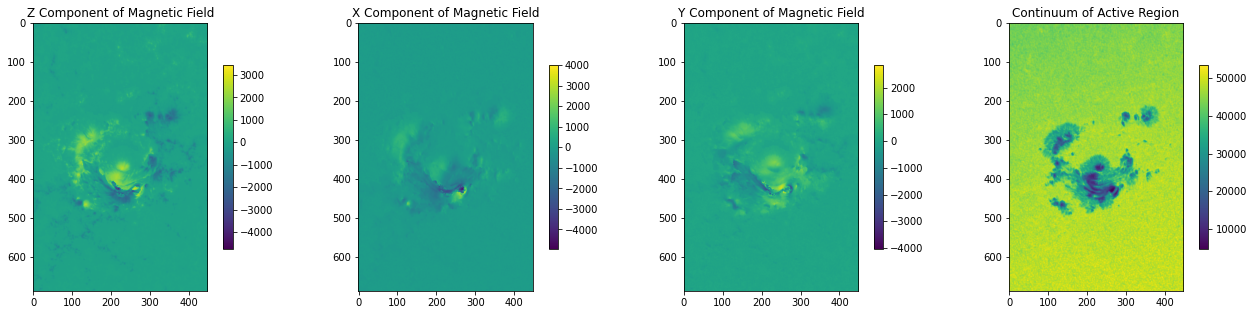
\includegraphics[width=\linewidth]{ThesisFilePkg/figures/data/activeregionfull.png}
\caption{The $x, y, z$ components of the magnetic field and continuum of SHARP AR number 7115 on 09/06/2017 at 12:00:00 UTC shown visually}
\label{activeregionall}
\end{figure}

These AR timeseries are standalone products that are not labeled flaring or non-flaring. The National Oceanic and Atmospheric Administration (NOAA) keeps a record of the size and duration of flares through time and matches individual SHARPs based on the relative timing and location on the solar disk. This combination of data product (magnetogram and continuum through the SHARP) and label (flaring or non-flaring through the NOAA SWPC record) forms a countable set of input-output pairs with a discrete answer space. Therefore, a ``flare forecasting" method (a function $f_{flare}$) as described in this paper will strictly be a classification problem, with a SHARP image set as an input (represented as a feature extracted vector) and a binary flaring or non-flaring as an output:
$$f_{flare} : \{\textit{Continuum} \in \mathbb{R}^{n\times m}, \textit{Magnetogram} \in \mathbb{R}^{3\times n \times m}\} \rightarrow \{\textit{Flaring}, \textit{Non Flaring}\}$$

In this study, I will use the data products generated by JSOC and extract four meaningful subregions from each of the image pair (Continuum, Magnetogram) called the Neutral Line, Umbra, Penumbra, and Background (described in detail in chapter \ref{chp:data}). I will then compute a list of physical and geometric parameters (58 real-valued scalars that describe physical properties of the AR) \textit{restricted to these subregions}. For example, I will compute the total magnetic flux \textit{within an umbra} instead of the net magnetic flux of the entire AR. At first, in my Segmented feature set, I will extract these features and stack the features of each subregion (a vector of size $4 \times 58 = 232$). Therefore, my ``input data" will reside in a $232$ dimensional vector space. I will also cluster subregions based on their pixel proximity and connect their clusters in the form of a graph (described in depth in chapter \ref{chp:data}) and use a graph neural network to classify the AR graphs as flaring or non-flaring. Finally, I will extract and average all 58 features from the entire AR to obtain a ``Full" feature set to see if segmenting improves my measures in my forecasting method. The distinction between the three feature sets is shown in figure \ref{fig:pipeline}. We begin with an AR image, chose to either segment it or leave it as is. The segmentation left as is is called the ``Full" feature set. The segmented region can either be left alone (``Segmented feature set") or turned into a graph (``graph feature set").
%%%%%%%%%%%%%
\begin{figure}[h]
    \centering
    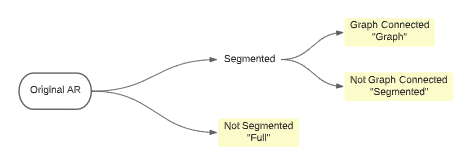
\includegraphics[width=0.8\linewidth]{ThesisFilePkg/figures/data/pipeline.png}
    \caption{The three (in yellow) main feature sets. This AR can either be segmented or not. When segmented, it can either be connected in the form of a graph or not. For each of these feature sets, the organization into a time series will not change the feature set, simply just an acknowledgment of the time stamp in whatever method.}
    \label{fig:pipeline}
\end{figure}

After I have extracted the four sub-regions' feature sets, I will create various supervised machine learning models to train on each feature set and compare the results of each model to see if there is an improvement from the Full or SHARPs feature sets. I chose a set of "simple" models (K nearest neighbors, naive Bayes, support vector machine, logistic regression, decision trees, and random forests) and attempted to classify input data points of the vector feature sets as ``M+ flaring" in the next 24 hours or ``M+ quiet" in the next 24 hours. I run each method multiple times and conclude that models trained on the Segmented feature set perform better (an average increase of 0.1 points in the True Skill Statistic) than the same models trained on the Full and SHARPs feature sets. I then design an Artificial Neural Network (ANN) to solve my second goal and show that by making minor fixes, I can optimize the model for functional flare prediction by weighing the importance of ARs closer to flaring in the loss function greater than ARs further from flaring (explained in more detail in chapter \ref{chaptermethods}).

My primary result is that models trained on the Segmented feature set perform better than models trained on either Full or SHARPs. This result satisfies my first goal laid out in the abstract. My second goal will not have any results; instead, I will attempt to explain some of the shortcomings of my models and the problem space as a whole to motivate future efforts in creating a more practical machine learning model to predict solar flares. I conclude that treating this problem as a binary classification problem has its shortcomings and that there are ways to fine-tune models to improve the confidence of short term predictions (and have a higher model performance the closer an input is to flaring).